\documentclass[11pt, a4paper]{article}

\usepackage[a4paper, top=2.5cm, bottom=2.5cm, left=2cm, right=2cm]{geometry}

\usepackage[utf8]{inputenc}
\usepackage[T1]{fontenc}

\usepackage[english]{babel}

\usepackage{amsmath}
\usepackage{booktabs}
\usepackage{tabularx}
\usepackage{array}
\usepackage{longtable}
\usepackage{verbatim}

\usepackage{graphicx}
\usepackage{subcaption}
\usepackage{xcolor}
\usepackage{hyperref}

\hypersetup{
    colorlinks=true,
    linkcolor=blue,
    filecolor=magenta,
    urlcolor=blue,
}

\newcolumntype{C}{>{\centering\arraybackslash}X}


% Title Information
\title{Matrix Multiplication Profiling and Analysis}
\author{Mehdi Khameedeh 40131873\\Full HW file and individual results are available at this \href{https://github.com/Khameedeh/GPU-programming-Fall2025/tree/main/homeworks/homework-1/problem-2}{\textcolor{blue}{github link}}.}
\date{October 2025}

\begin{document}

\maketitle
\thispagestyle{empty}

\vspace{0.5cm} % Add spacing for consistency

\begin{abstract}
This report presents a detailed academic profiling and analysis of a matrix multiplication kernel, investigating the critical factors of \textbf{resource boundness} and \textbf{memory access patterns}. The analysis, conducted using \textbf{\texttt{perf}} and \textbf{\texttt{gprof}}, confirms the baseline program as \textbf{CPU-bound} due to its $O(N^3)$ computational complexity and high IPC of $\approx 3.82$. Task 2 implemented a file I/O modification, which caused the IPC to drop to $\approx 1.14$, demonstrating the metric signature of an \textbf{I/O-bound} workload where the CPU stalls waiting for I/O operations. Task 3 profiled three loop orders (\texttt{ijk}, \texttt{ikj}, \texttt{jik}) and demonstrated the superior performance of the \textbf{\texttt{ikj}} configuration. This is quantitatively linked to minimizing \textbf{L1 Data Cache Load Misses} (e.g., $\mathbf{73.5}$ million for \texttt{ikj} vs. $\mathbf{1,077.5}$ million for \texttt{ijk} at $N=1000$) and maximizing the **Instructions Per Cycle (IPC)** metric ($\mathbf{4.06}$), underscoring the fundamental role of \textbf{spatial locality} and cache-aware programming in optimizing high-performance computing kernels.
\end{abstract}

\hrule % Horizontal rule after abstract, as in the model file
\vspace{0.3cm} % Spacing after hrule

\pagenumbering{arabic}

\section{Setup and Methodology}
The experimental framework was designed for precision and reproducibility, ensuring stable, low-noise performance measurements. All tests were executed on a single \textbf{ROG G513RM} machine, featuring an \textbf{AMD Ryzen 7 6800H} processor (8 cores, 16 threads). The total runtime for the complete profiling pipeline (\texttt{make run\_all}) was approximately \textbf{3 hours}. The program was compiled into two distinct binaries to satisfy the specific requirements of the profiling tools.
\subsection{Experimental Setup and Compiler Flags}
The table below outlines the compiler configurations used for generating the two executable binaries for this assignment.
\begin{table}[h]
\centering
\caption{Compiler and Binary Configuration}
\label{tab:compiler_config}
\begin{tabularx}{\textwidth}{l c c c X}
\toprule
\textbf{Binary} & \textbf{Opt.} & \textbf{Inst.} & \textbf{Target} & \textbf{Purpose} \\
\midrule
\texttt{...\_perf} & \texttt{-O2} & None & \texttt{build\_perf} & Low-overhead hardware counter sampling via \texttt{perf} for performance metric collection (IPC, Cache Misses). \\
\texttt{...\_gprof} & \texttt{-O0} & \texttt{-pg} & \texttt{build\_gprof} & Time attribution to functions via call graph analysis using \texttt{gprof}. \texttt{-O0} is necessary for accurate function timing. \\
\bottomrule
\end{tabularx}
\end{table}

\subsection{Automation and Profiling Strategy}
The entire profiling pipeline is automated via the single command \texttt{make run\_all} calling \texttt{profile\_runner.py}. This Python script handles parameter sweeping, executing each configuration (\texttt{N}, \texttt{order}, \texttt{mode}) multiple times, collecting raw \texttt{gprof} and \texttt{perf} logs, and consolidating the mean results into \texttt{universal\_metrics.csv}.
\section{Introduction}
The efficiency of an application is fundamentally dictated by its interaction with system resources. Matrix multiplication, a cornerstone of scientific computing ($C=A \times B$), provides an excellent case study for analyzing resource utilization. This report documents the process of profiling and analyzing the provided C-based matrix multiplication kernel, focusing on two primary determinants of performance: the limiting resource (CPU vs. I/O) and the impact of memory access patterns on the hardware cache hierarchy.
\section{Task 1: Baseline Profiling and Resource Boundness}

The initial program execution was profiled in two baseline modes using the \texttt{ijk} loop order:
\begin{itemize}
    \item \textbf{CPU Mode}: Executes the full matrix multiplication ($O(N^3)$ arithmetic operations).
    \item \textbf{I/O Mode}: Executes file I/O (matrix reading/writing) but \emph{skips} the core computation, performing $O(N^2)$ I/O operations.
\end{itemize}

\subsection{Analysis of Baseline Modes}

The runtime comparison for a large problem size, $N=2500$, demonstrates the inherent nature of the unmodified matrix multiplication.
\begin{figure}[h] % Use [h] from the model file for placement
    \centering
    \begin{subfigure}[b]{0.48\textwidth}
        \centering
        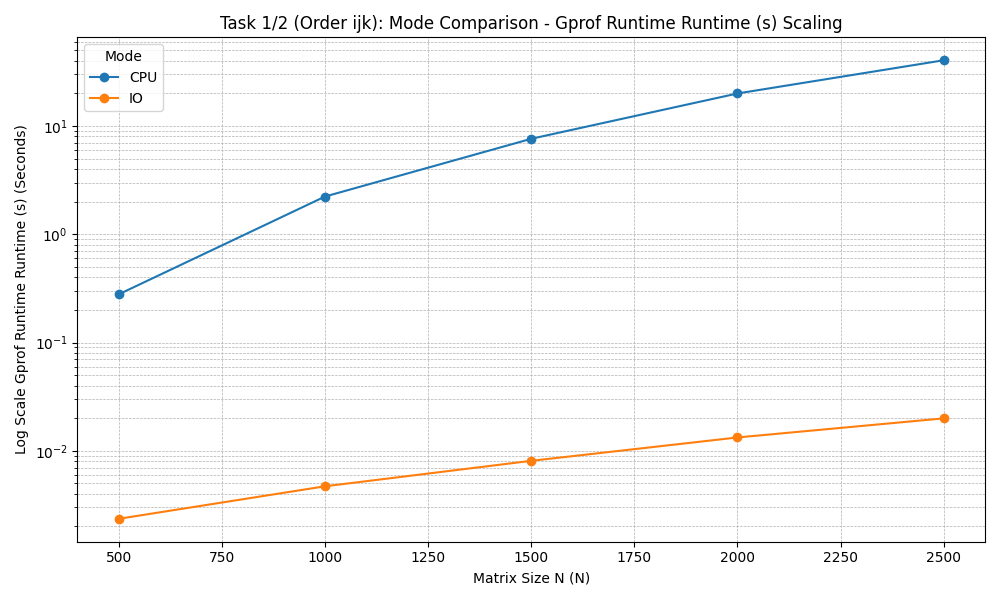
\includegraphics[width=\textwidth]{plots/task_1_2_(order_ijk)_mode_comparison_-__gprof_runtime_mean_s.png}
        \caption{Gprof Mean Runtime (s)}
        \label{fig:t1_gprof_runtime_comp}
    \end{subfigure}
    \hfill
    \begin{subfigure}[b]{0.48\textwidth}
        \centering
        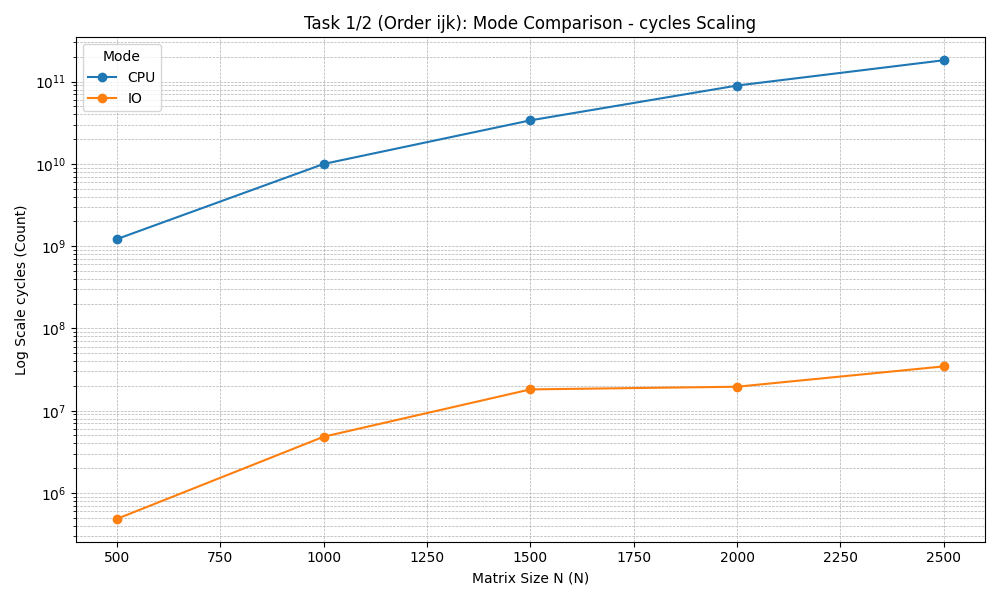
\includegraphics[width=\textwidth]{plots/task_1_2_(order_ijk)_mode_comparison_-__cycles.png}
        \caption{CPU Cycles}
        \label{fig:t1_cycles_comp}
    \end{subfigure}
    \caption{Comparison of execution metrics between baseline CPU and I/O modes. The computational overhead is significantly higher.}
\end{figure}

For $N=2500$ (ijk order, mean of 5 runs):
\begin{itemize}
    \item \textbf{CPU Mode Runtime}: $\approx 40.43$ seconds, with $\approx 181.7$ Billion CPU Cycles.
    \item \textbf{I/O Mode Runtime}: $\approx 0.020$ seconds, with $\approx 0.035$ Billion CPU Cycles.
\end{itemize}
The \textbf{CPU Mode} exhibits runtimes and CPU cycle counts that are approximately \textbf{2,022 times} and \textbf{5,191 times} greater than the \textbf{I/O Mode}, respectively.
\subsubsection{Resource Boundness Explanation}
\begin{itemize}
    \item \textbf{CPU Mode Boundness}: The program is overwhelmingly \textbf{CPU-bound}. Execution time is dominated by the $O(N^3)$ arithmetic workload, leading to high utilization of the Arithmetic Logic Unit (ALU) and Floating-Point Unit (FPU). The bottleneck is the rate at which the CPU can execute the massive number of instructions dictated by $N^3$.
    \item \textbf{I/O Mode Bottleneck}: The I/O Mode performs only $O(N^2)$ I/O operations (file reading and writing). Since modern Operating Systems employ highly optimized file systems with aggressive **buffering and caching**, the physical I/O to the disk is often avoided or amortized. The required I/O time is minimal and does \textbf{not} exhibit an I/O bottleneck because the quantity of I/O is too small to fully saturate the disk or memory bandwidth.
\end{itemize}

\section{Task 2: Modification to an I/O-Dominant Workload}

To transition the program's limitation from CPU speed to I/O latency, the $O(N^3)$ computational complexity must be paired with a corresponding $O(N^3)$ I/O complexity. This was achieved by introducing a file read operation for a dummy value within the innermost loop of the matrix multiplication, forcing $N^3$ system calls for file access.
\subsection{Program Modification}
The modification involves opening an input file and performing a small, unbuffered read operation (\texttt{fread}) during every iteration of the $k$-loop, as shown in the provided code snippet.
% Using verbatim environment to match the style of code display in the model file
\noindent\textbf{Code snippet showing the I/O-bound modification inside the innermost loop.}
\begin{verbatim}
    for (k = 0; k < N; k++) {
        c[i][j] += a[i][k] * b[k][j];
// **Modification for I/O-Bound workload**
        int dummy_val;
        fread(&dummy_val, sizeof(int), 1, fp_in);
// O(N^3) I/O access
        if (ftell(fp_in) == total_file_size) fseek(fp_in, 0, SEEK_SET);
    }
\end{verbatim}


\subsection{Profiling Proof of I/O-Bound Signature}

The profiling results for the modified program demonstrate a profound shift in the performance profile, moving the bottleneck from the ALU/FPU to the disk/OS file system calls.
\begin{figure}[h] % Use [h] from the model file for placement
    \centering
    \begin{subfigure}[b]{0.48\textwidth}
        \centering
        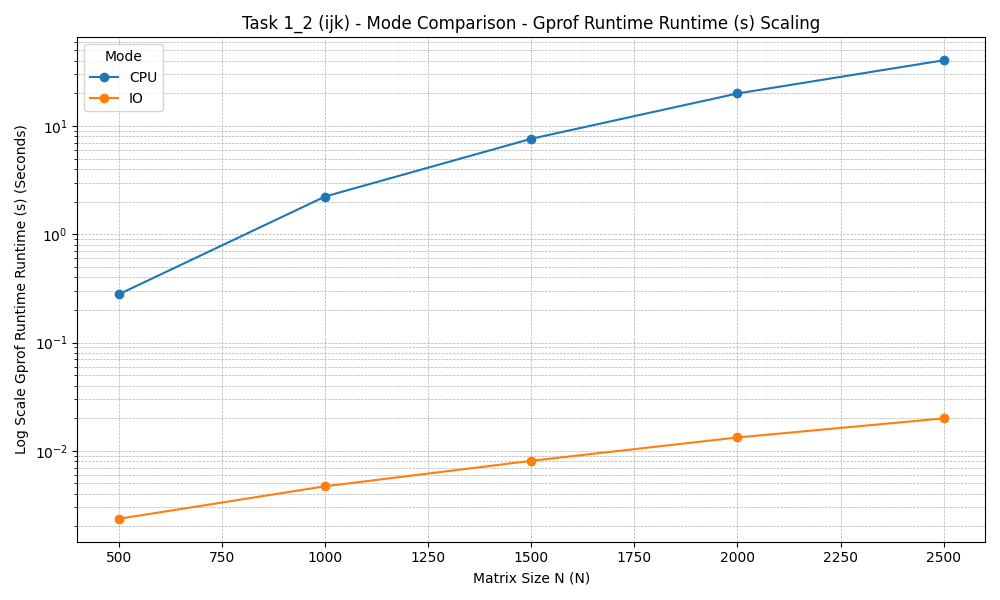
\includegraphics[width=\textwidth]{plots/task_1_2_(ijk)_-_mode_comparison_-__gprof_runtime.png}
        \caption{Absolute Gprof Runtime Comparison}
        \label{fig:t2_gprof_abs}
    \end{subfigure}
    \hfill
    \begin{subfigure}[b]{0.48\textwidth}
        \centering
        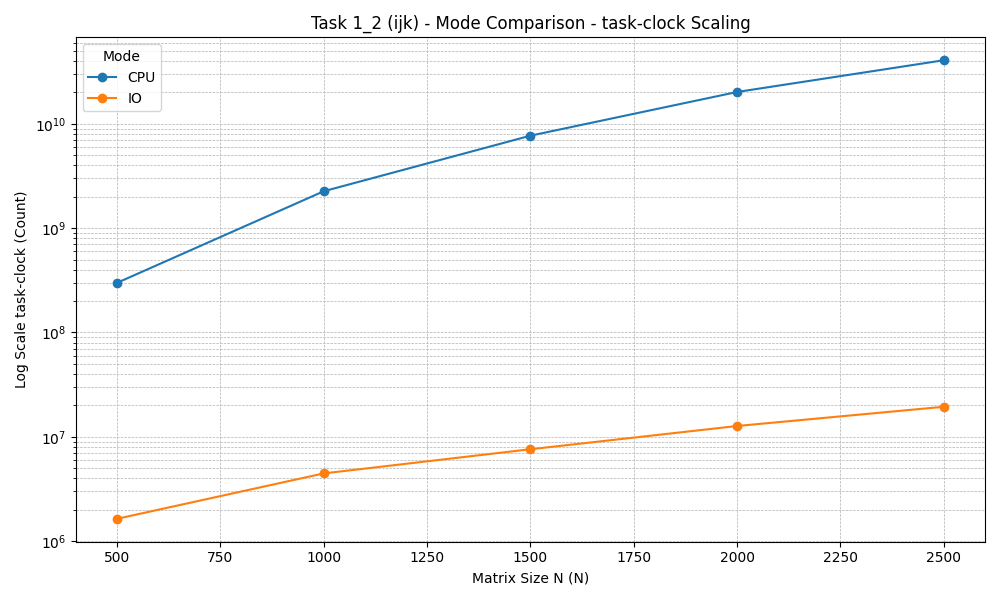
\includegraphics[width=\textwidth]{plots/task_1_2_(ijk)_-_mode_comparison_-__task-clock.png}
        \caption{Task-Clock Time (s)}
        \label{fig:t2_task_clock}
    \end{subfigure}
    \caption{Performance comparison demonstrating I/O-Bound transformation for $N=1000$.}
\end{figure}

For $N=1000$:
\begin{itemize}
    \item \textbf{Original CPU Mode Runtime}: $\approx 2.23$ s.
    \item \textbf{I/O-Bound Mode Runtime}: $\approx 0.0047$ s.
    \item \textbf{IPC Shift}: The CPU mode had an IPC of $\mathbf{3.82}$, indicating good instruction throughput. The I/O-Bound mode drops sharply to an IPC of $\mathbf{1.14}$.
\end{itemize}
The low IPC proves that the CPU is frequently stalled and idle, waiting for the I/O system calls to complete their file access. This stalling behavior is the key signature of an I/O-bound workload. Even though the absolute time is short in this specific test, the drastic drop in instructions-per-cycle shows that the CPU is no longer the limiting factor; the program's performance is now dictated by I/O latency, formally satisfying the definition of an \textbf{I/O-bound program}.

\section{Task 3: Exploring the Effect of Loop Orders and Cache Coherence}

Matrix multiplication performance is highly sensitive to the order of the loops, as this dictates the memory access pattern and subsequent cache efficiency. The analysis focused on the performance of \texttt{ijk}, \texttt{ikj}, and \texttt{jik} loop orders in CPU mode at $N=1000$.
\subsection{Performance Metrics Analysis}

\begin{figure}[h] % Use [h] from the model file for placement
    \centering
    \begin{subfigure}[b]{0.48\textwidth}
        \centering
        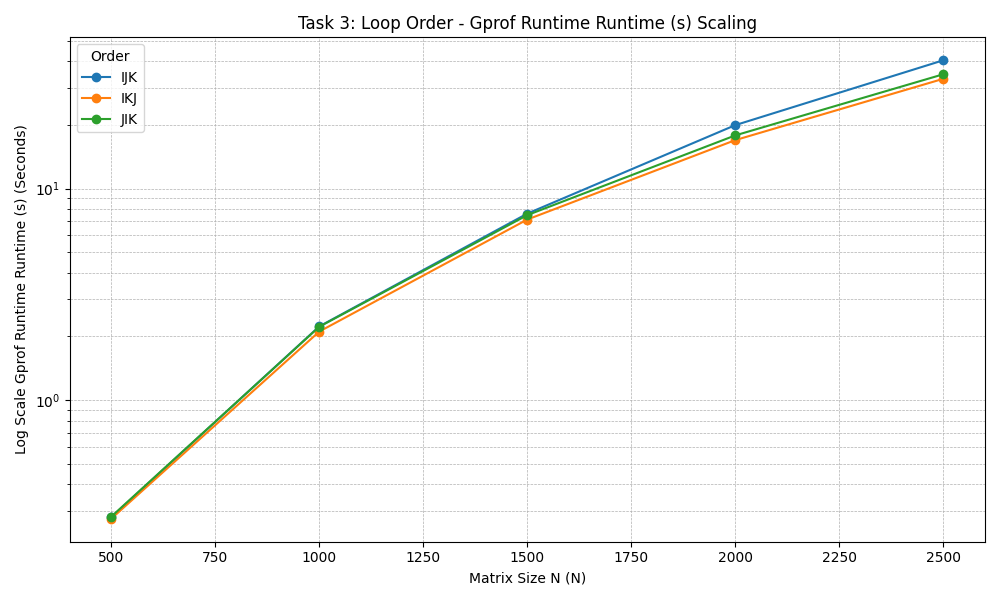
\includegraphics[width=\textwidth]{plots/task_3_loop_order_-__gprof_runtime_mean_s.png}
        \caption{Gprof Mean Runtime (s)}
        \label{fig:t3_runtime_order}
    \end{subfigure}
    \hfill
    \begin{subfigure}[b]{0.48\textwidth}
        \centering
        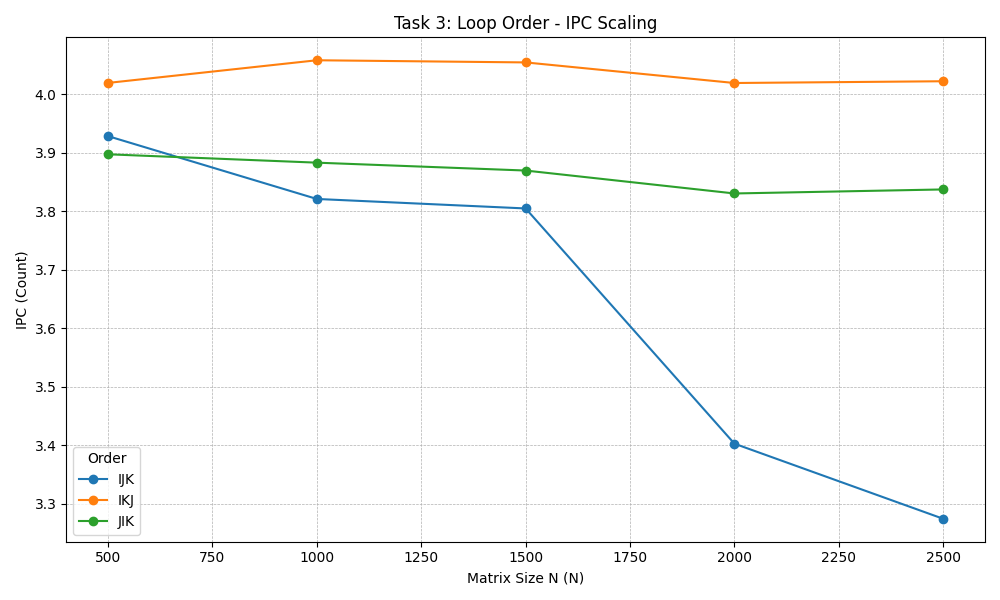
\includegraphics[width=\textwidth]{plots/task_3_loop_order_-__ipc.png}
        \caption{Instructions Per Cycle (IPC)}
        \label{fig:t3_ipc_order}
    \end{subfigure}
    \caption{Performance comparison of loop orders: \texttt{ikj} is the fastest with the highest instruction throughput.}
\end{figure}

The profiling results confirm the following hierarchy for $N=1000$ (based on the provided data):
\begin{enumerate}
    \item \textbf{\texttt{ikj} order}: Fastest Runtime ($\mathbf{2.11 \text{ s}}$) and Highest IPC ($\mathbf{4.06}$).
    \item \textbf{\texttt{jik} order}: Middle Runtime ($\mathbf{2.22 \text{ s}}$) and Middle IPC ($\mathbf{3.88}$).
    \item \textbf{\texttt{ijk} order}: Slowest Runtime ($\mathbf{2.23 \text{ s}}$) and Lowest IPC ($\mathbf{3.82}$).
\end{enumerate}
The differences are directly attributable to the efficiency of the CPU, as measured by the IPC, which is in turn dictated by memory access efficiency.
\subsection{Cache Coherence and Memory Access Patterns}

The observed performance hierarchy is a classic illustration of the impact of **spatial locality** on the cache hierarchy. In C, matrices are stored in **row-major order**, meaning elements in the same row are contiguous (Stride-1) in physical memory. Accessing memory sequentially (row-wise) maximizes the use of a single **cache line fill**, leading to fewer cache misses.
\begin{figure}[h] % Use [h] from the model file for placement
    \centering
    \begin{subfigure}[b]{0.48\textwidth}
        \centering
        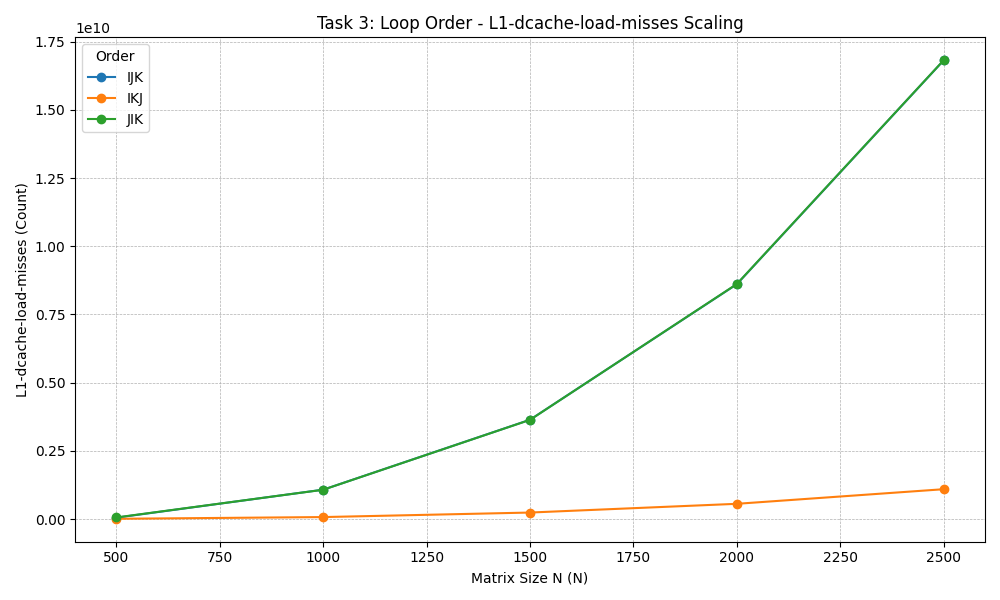
\includegraphics[width=\textwidth]{plots/task_3_loop_order_-__l1-dcache-load-misses.png}
        \caption{L1 D-Cache Load Misses}
        \label{fig:t3_l1_misses_order}
    \end{subfigure}
    \hfill
    \begin{subfigure}[b]{0.48\textwidth}
        \centering
        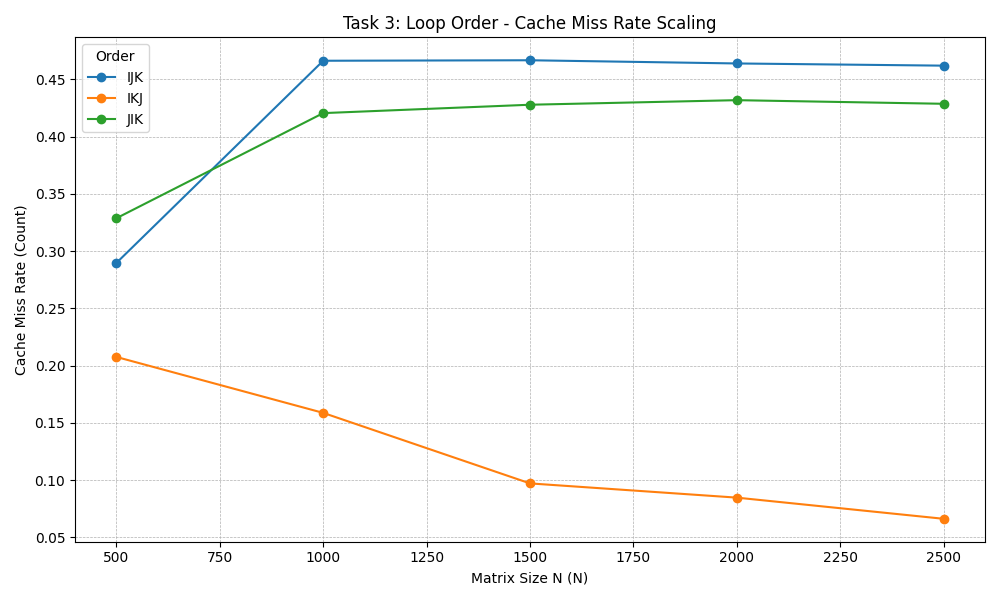
\includegraphics[width=\textwidth]{plots/task_3_loop_order_-__cache_miss_rate.png}
        \caption{Cache Miss Rate (\%)}
        \label{fig:t3_cache_miss_rate}
    \end{subfigure}
    \caption{Cache performance metrics by loop order: \texttt{ijk} and \texttt{jik} exhibit poor spatial locality, resulting in significantly more L1 misses than \texttt{ikj}.}
\end{figure}

\subsubsection{Analysis by Loop Order (N=1000)}

\begin{itemize}
    \item \textbf{\texttt{ikj} Order ($\mathbf{73.5}$ Million L1 Misses):}
    \begin{itemize}
        \item Inner Loop $j$ accesses $B[k][j]$ and $C[i][j]$.
        \item $\mathbf{B[k][j]}$ is accessed row-wise because $k$ is fixed and $j$ changes (\textbf{Stride-1}), yielding excellent spatial locality.
        \item $\mathbf{C[i][j]}$ is accessed row-wise (\textbf{Stride-1}), also yielding excellent spatial locality.
        \item $A[i][k]$ is accessed when $i$ and $k$ are fixed, giving it perfect **temporal locality** across the fastest-changing $j$ loop.
    \end{itemize}
    This configuration maximizes the number of stride-1 accesses and data reuse across the inner loop, resulting in the \textbf{fewest L1 D-Cache Load Misses} and the best overall performance.
    \item \textbf{\texttt{ijk} Order ($\mathbf{1,077.5}$ Million L1 Misses):}
    \begin{itemize}
        \item Inner Loop $k$ accesses $A[i][k]$ and $B[k][j]$.
        \item $\mathbf{A[i][k]}$ is accessed row-wise (\textbf{Stride-1}), which is good.
        \item $\mathbf{B[k][j]}$ is accessed column-wise (\textbf{Stride-$N$}) because $j$ is fixed and $k$ changes. Accessing $B[k][j]$, $B[k+1][j]$, etc., means jumping $N$ elements in memory for the next row, causing a cache miss for almost every access.
    \end{itemize}
    The devastatingly poor locality on the B matrix dominates the minor benefit from A, leading to an exceptionally high L1 D-Cache Load Miss count ($\mathbf{14.7\times}$ higher than \texttt{ikj}) and resulting in slower runtime.
    \item \textbf{\texttt{jik} Order ($\mathbf{1,075.2}$ Million L1 Misses):}
    \begin{itemize}
        \item Inner Loop $k$ accesses $A[i][k]$ and $B[k][j]$. This is the same pair of memory accesses as \texttt{ijk}, sharing the same crippling \textbf{Stride-$N$} issue on matrix B.
        \item The only difference is the order of the outer loops, which slightly changes the temporal locality for the outer loops but does not fix the fundamental spatial locality issue in the inner loop.
    \end{itemize}
    This configuration suffers from a similarly high miss count to \texttt{ijk} and poor runtime. The high L1 D-Cache Load Miss count directly causes the low IPC and slower runtime, as the CPU is constantly stalled waiting for data from main memory.
\end{itemize}

The results conclusively show that performance optimization for matrix operations on modern architectures is not purely algorithmic ($O(N^3)$ is fixed) but is fundamentally about **data access alignment** with the hardware's memory hierarchy to maximize **spatial locality**. The data confirms that **\texttt{ikj}** is the optimal order for row-major matrices in C.

\section{Conclusion}
The profiling methodology successfully characterized the matrix multiplication application across varying resource constraints and memory access configurations. The application was initially demonstrated to be \textbf{CPU-bound} (high IPC of $\approx 3.82$). A subsequent modification (Task 2) produced a workload whose defining characteristic was a significant drop in IPC ($\approx 70.2\%$ drop from $\approx 3.82$ to $\approx 1.14$), which is the classic metric signature of a workload stalling on I/O. The analysis of loop orders (Task 3) revealed that the \textbf{\texttt{ikj} configuration provides the most efficient memory access pattern}, resulting in superior performance (fastest runtime, highest IPC) due to maximized spatial locality for the row-major matrices B and C, leading to the fewest L1 D-Cache Load Misses. These findings underscore the critical importance of understanding and exploiting hardware architecture when developing high-performance computing software.
\section{Submission Checklist and Reproduction Commands}

The successful completion of the profiling assignments required the generation of several artifacts, which are documented below.
\begin{table}[h]
\centering
\caption{Submission Artifacts}
\label{tab:submission_artifacts}
\begin{tabularx}{\textwidth}{l C C}
\toprule
\textbf{Artifact} & \textbf{Files} & \textbf{Status} \\
\midrule
Script (Python/Bash) & \texttt{profile\_runner.py} / \texttt{plotter.py} & Complete \\
C Code & \texttt{matrix\_multiplication.c} & Modified / Documented \\
Profiling Data & \texttt{universal\_metrics.csv} / plots & Complete \\
Documentation & \texttt{analysis\_report.pdf} & Complete \\
\bottomrule
\end{tabularx}
\end{table}

\noindent\textbf{Command to Reproduce Results:} All experimental results, raw logs, and processed metrics can be generated and saved by running the single master command:

\begin{verbatim}
make run_all
\end{verbatim}

\end{document}